
\documentclass[letterpaper,11pt,titlepage,final]{report}

\usepackage{epsfig,pifont,calc,color,pstricks}
\usepackage{amsmath,latexsym,oldlfont}
\usepackage{enumerate}
\usepackage{Chicago}
\usepackage{url}

\usepackage{graphicx, animate}
\usepackage{caption}

\def\MonthYear{\today}

%%%%%%%%%%%%%%%%%%%%%%%%%%%%
%% A4 wide
%%%%%%%%%%%%%%%%%%%%%%%%%%%%
 
\usepackage{a4wide}
%\textwidth 16.7cm
%\textheight 24.6cm
%\oddsidemargin -4.5mm
%\evensidemargin -4.5mm
%\topmargin -11.5mm
 
%%%%%%%%%%%%%%%%%%%%%%%%%%%%
%% US letter
%%%%%%%%%%%%%%%%%%%%%%%%%%%%
 
%\textwidth 17cm
%\textheight 23.8cm
%\oddsidemargin -4.5mm
%\evensidemargin -4.5mm
%\topmargin -22.5mm
 
%%%%%%%%%%%%%%%%%%%%%%%%%%%%

%\usepackage{fancyheadings}
\usepackage{fancyhdr}
\pagestyle{fancyplain}
\renewcommand{\chaptermark}[1]{\markboth{#1}{#1}}
\renewcommand{\sectionmark}[1]{\markright{\thesection\ #1}}
\lhead[\fancyplain{}{\bfseries\thepage}]{\fancyplain{}{\bfseries\rightmark}}
\rhead[\fancyplain{}{\bfseries\leftmark}]{\fancyplain{}{\bfseries\thepage}}
\cfoot{}
\renewcommand{\labelitemii}{{\LARGE\bf .}}

% pour voir la bounding box postscript
%\newcommand{\voirbbox}[1]{{\fboxsep 0pt \fbox{#1}}}

% pour ne pas la voir
\newcommand{\voirbbox}[1]{{{#1}}}

%
% define new items (necessite package pifont)
%

\font\pzdr=pzdr at 12pt

\newenvironment{fancyitemize}[1]
   {\begin{itemize}
    \renewcommand{\labelitemi}{{\pzdr #1}}
    \renewcommand{\labelitemii}{{\pzdr #1}}
    \renewcommand{\labelitemiii}{{\pzdr #1}}
   }
   {\end{itemize}}

%
% define new enumerate (necessite package pifont et calc)
%

\newcounter{local}

\newenvironment{enumerateW}
   {
     \begin{enumerate}
     \renewcommand{\labelenumi}{\setcounter{local}{191+\value{enumi}}\ding{\value{local}}}
     \renewcommand{\labelenumii}{\setcounter{local}{191+\value{enumii}}\ding{\value{local}}}
     \renewcommand{\labelenumiii}{\setcounter{local}{191+\value{enumiii}}\ding{\value{local}}}
   }
   {\end{enumerate}}

\newenvironment{enumerateB}
   {
     \begin{enumerate}
     \renewcommand{\labelenumi}{\setcounter{local}{201+\value{enumi}}\ding{\value{local}}}
     \renewcommand{\labelenumii}{\setcounter{local}{201+\value{enumii}}\ding{\value{local}}}
     \renewcommand{\labelenumiii}{\setcounter{local}{201+\value{enumiii}}\ding{\value{local}}}
   }
   {\end{enumerate}}

\newcommand{\relief}[1]{{\it\bfseries #1}}

%%%%%%%%%%%%%%%%%%%%%%%%%%%%%%%%%%%%%%%%%%%%%%%%%%%%%%%%%%%%%%%%%%
% FIGURES:

\newcommand{\Img}[2]{
\begin{minipage}{#2\linewidth}
\centerline{ \epsfig{file=\ImPath/#1,width=\linewidth}}
\end{minipage}
}

\newcommand{\ImgC}[2]{
\centerline{ \epsfig{file=\ImPath/#1,width=#2\linewidth} }
}

\newcommand{\ImgL}[2]{
\begin{minipage}{#2\linewidth}
\centerline{ \epsfig{file=\ImPath/#1,width=\linewidth,angle=-90}}
\end{minipage}
}

\newcommand{\ImgCL}[2]{
\centerline{ \epsfig{file=\ImPath/#1,width=#2\linewidth,angle=-90} }
}

%%%%%%%%%%%%%%%%%%%%%%%%%%%%%%%%%%%%%%%%%%%%%%%%%%%%%%%%%%%%%%%%%%%%%
% EQUATIONS:
\newcommand{\eq}{\begin{equation}}
\newcommand{\en}{\end{equation}}
\newcommand{\eqa}{\begin{eqnarray}}
\newcommand{\ena}{\end{eqnarray}}

%%%%%%%%%%%%%%%%%%%%%%% REFERENCES %%%%%%%%%%%%%%%%%%%%%%%%%%%%%%%%%%%
\newcommand{\Eqref}[1]{Equation~\ref{Eq:#1}}
\newcommand{\figref}[1]{Figure~\ref{Fig:#1}}
\newcommand{\secref}[1]{Section~\ref{Sec:#1}}
\newcommand{\charef}[1]{Chapter~\ref{Cha:#1}}
\newcommand{\appref}[1]{Appendix~\ref{App:#1}}
\newcommand{\tabref}[1]{Table~\ref{Tab:#1}}

%%%%%%%%%%%%%%%%%%%%%%%%%%%%%%%%%%%%%%%%%%%%%%%%%%%%%%%%%%%%%%%%%%%%%
% SHORTER ITEMIZE
\newenvironment{sitemize}
{\begin{list}{--}%
  {\setlength{\topsep}{0pt}%
   \setlength{\itemsep}{0pt}%
   \setlength{\leftmargin}{2em} }}
{\end{list}}

\newenvironment{senumerate}
{\begin{enumerate}
  \setlength{\topsep}{0pt}
  \setlength{\itemsep}{0pt}
  \setlength{\parskip}{0pt}
  \setlength{\parsep}{0pt}}
{\end{enumerate}
}

%%%%%%%%%%%%%%%%%%%%%%%%%%%%%%%%%%%%%%%%%%%%%%%%%%%%%%%%%%%%%%%%%%%%%

%\includeonly{chap1}

%
% Start the Report
%
\begin{document}

\parindent 0pt
\parskip 10pt

%%%%%%% TITLE PAGE %%%%%%%%%%%%%%%%%%%%%%%%%%%%%%%

\thispagestyle{empty}
\vspace*{\fill}
\begin{center}

%\pspicture(15.5,0)
%\psline[linestyle=solid,linecolor=red,linewidth=2pt](-0.1,0)(15.6,0)
%\endpspicture

\vspace*{1mm}
{\Huge\bf{ Extended-source modeling in SEM3D}}\\[2mm]
{\Large starting from Ruiz's kinematic-source model  }\\[5mm]
{\Large \bf{User's Guide}}


%\pspicture(15.5,0)
%\psline[linestyle=solid,linecolor=red,linewidth=1.5pt](-0.1,0.2)(15.6,0.2)
%\endpspicture



\newfont{\fdunB}{cmdunh10 scaled \magstep2}
\vspace*{3cm}
\fdunB
%Version \Version \\[3mm]
\MonthYear \\[3cm]
\end{center}
\vfill
%\newpage
\thispagestyle{empty}
\hspace*{0pt}
\newpage
\thispagestyle{empty}
\vspace*{\fill}

%%%%%%% TABLE OF CONTENTS %%%%%%%%%%%%%%%%%%%%%%%%%%%%%%%%%%%%%%%%%%%%%%

\newpage
{\parskip 0pt
  \tableofcontents
}
\newpage

%%%%%%% BODY %%%%%%%%%%%%%%%%%%%%%%%%%%%%%%%%%%%%%%%%%%%%%%%%%%%%%

\chapter{RIK model}
\label{chapRIK}


RIK (Ruiz's Integral Kinematic) model is an advanced kinematic source model developed by \cite{Ruiz2011} and further modified by \cite{Gallovic2016}. This method allows taking into account frequency-dependent directivity effects. The asperities have a fractal distribution that may follow a given inverted slip distribution. \\


The kinematic source model could be generated by using the RIKsrf code. It is provided in RIK\textunderscore MODEL/CODE\textunderscore GALLOVIC\textunderscore RIKsrf/ folder of the materials of this manual. Its compilation is verified for gfortran and ifort compilers. Two different sub-folders are available depending on compiler selection. Inside the selected sub-folder, the user should just run 'lancer.sh' file in order to compile the code, which creates the executable 'RIKsrf2'. \\ 


RIKsrf code works by calling the executable RIKsrf2 from any example folder. In this manual, a case from South Napa fault model is used as an example. The related folder to this example is 'RIK\textunderscore MODEL/EXAMPLES/NAPA\textunderscore ROCHER/'. Two input files are needed to run the RIKsrf code. The first one is 'RIKsrf.in'. The 'RIKsrf.in' file for Napa example is shown in the figure below:


%% FIGURE : RIKsrf.in
\begin{center}
\leavevmode
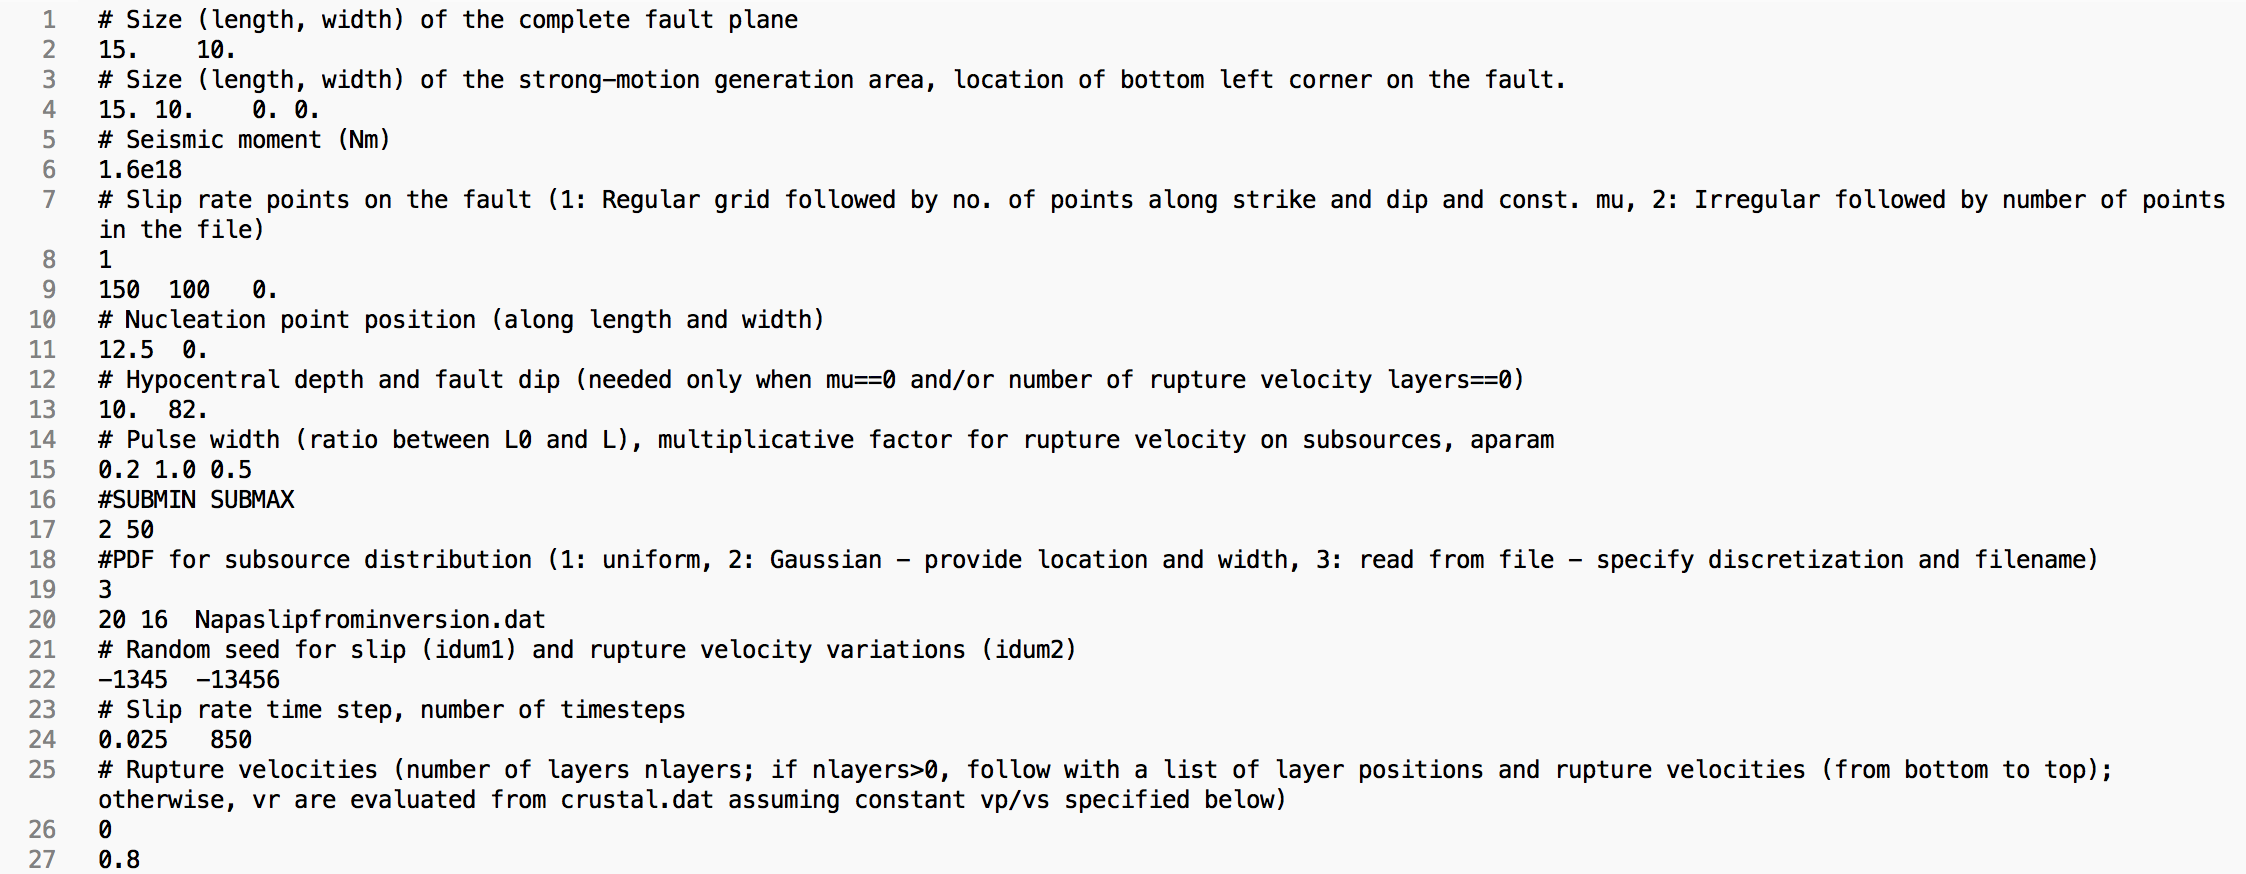
\includegraphics[scale=0.45]{figures/RIK-input1.png} 
\captionof{figure}{RIKsrf.in file for RIK model}
\label{rik1} 
\vspace{1cm}
\end{center}



In line 2, we define the size of fault plan (length and width). For our example, length is equal to 15 km and width is 10 km. The strong-motion generation area is the same as the complete fault plan. Thus, in line 4, we enter 15 and 10 for strong-motion generation area and the location of left bottom point. \\

In line 6, seismic moment is given in Nm. \\

In lines 8-9, we specify the choice of grid model. If a regular model is desired, 1 is written in line 8 and followed by the point number along strike and dip. Otherwise, the grid is determined by a given file. In our example, we work with a regular grid. In line 9, after point numbers, a constant rigidity value is specified. Since it is not used in this example, we write 0.  \\

In line 11, we define the location of hypocenter in fault plan. In our test, it is located at (12.5, 0). \\


In line 13, hypocenter depth and dip angle are written. \\


In line 15, impulse characteristics are defined based on \cite{Ruiz2011} model. For more details, please refer to \cite{Ruiz2011} and \cite{Gallovic2016}. \\


In line 17, the upper and lower limits that determine the size-distribution of asperities (sub-sources) are defined. \\

In lines 19-20, we specify the choice of slip-inversion data. In our example, we provide inverted slip distribution for Napa model so that in line 19 we enter 1 and in line 20 the file name is given. \\


In line 22, random seed for slip and rupture velocities are set. \\

In line 24, the time step and total duration for slip-velocity time histories are specified. \\

Lastly, in line 26, we define rupture velocities of layers in the model. Either one line is devoted to the property of each layer either it is provided by another file named 'crustal.dat'. In our case, we give another file. For such cases where 'crustal.dat' is used, a constant value (0.8 in this example) is set for rupture-to-shear velocity ratio. \\


In the following, we explain the content of 'crustal.dat' file in our example, Figure \ref{rik2}.



%% FIGURE : RIKsrf.in
\begin{center}
\leavevmode
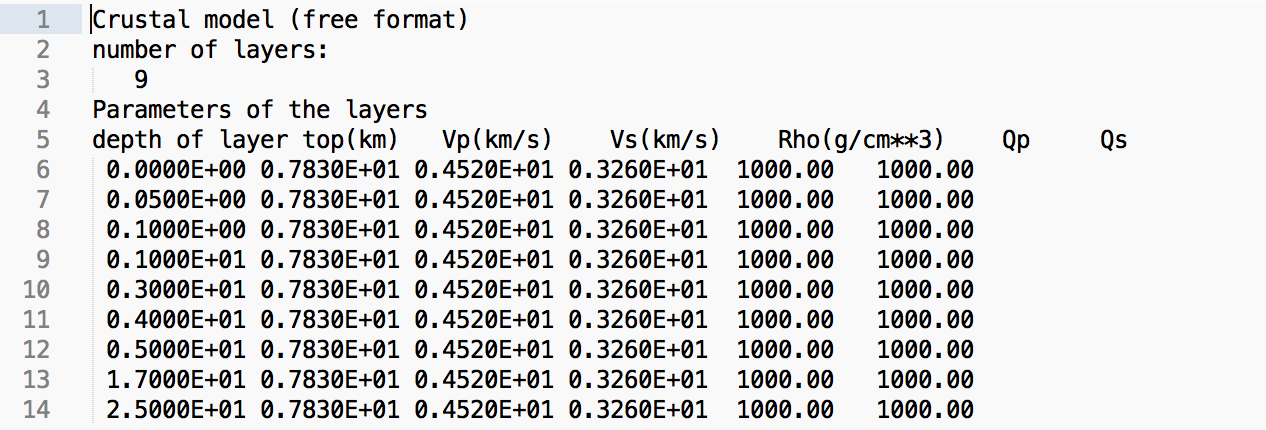
\includegraphics[scale=0.45]{figures/RIK-input2.png} 
\captionof{figure}{crustal.dat file for RIK model}
\label{rik2} 
\vspace{1cm}
\end{center}



First, in line 3, total number of layers is given. Then, starting from line 6, for each layer in the model, the depth of top level (positive in downward), pressure and shear wave velocities, density and quality factors for pressure and shear waves are defined. \\


After the simulation, the code sorts a number of output files such as slipdistribution.dat, subsources.dat etc. In RIK\textunderscore MODEL/EXAMPLES/python folder, two Python scripts are provided to plot maximum-slip distribution and asperity distribution on fault plan (slip.py and subsources.py respectively). For our example, the resultant figures for maximum-slip distribution and asperity distribution are given in Figures \ref{rik3}-\ref{rik4}.\\




%% FIGURE : RIKsrf.in
\begin{center}
\leavevmode
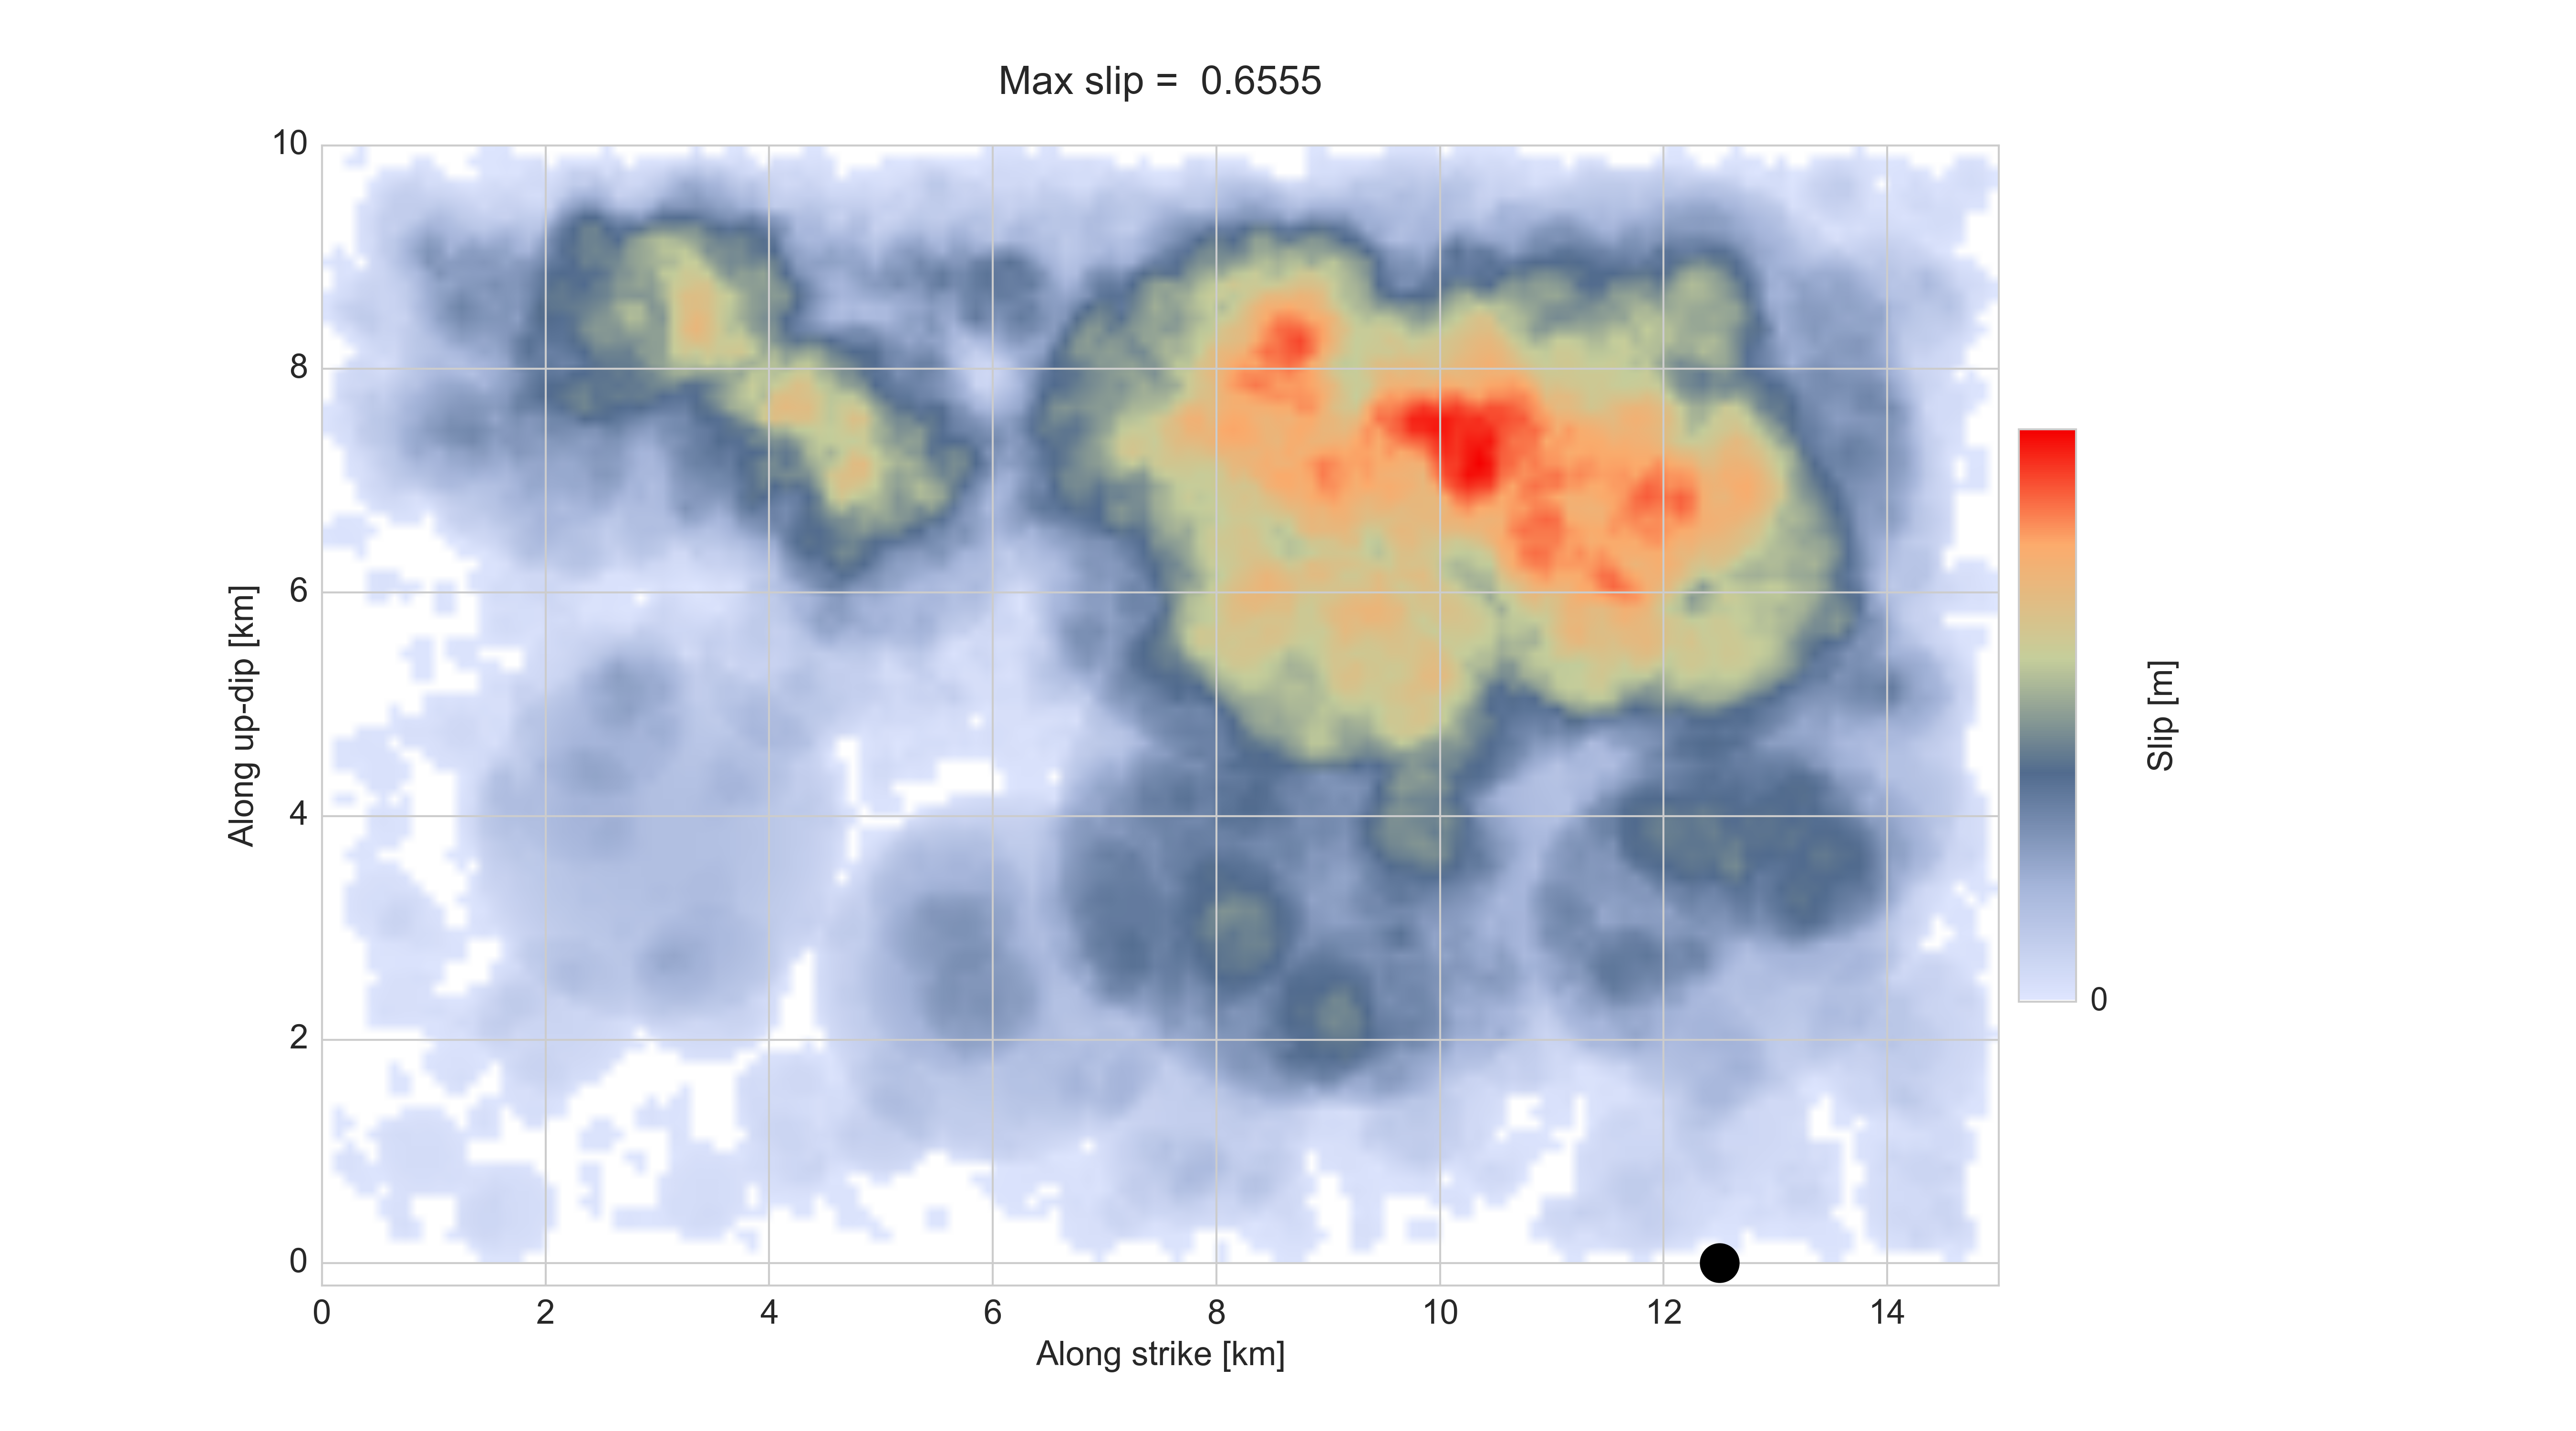
\includegraphics[scale=0.35]{figures/15000points_Napa_rocher_slip.png} 
\captionof{figure}{Maximum-slip distribution on fault plan of Napa event.}
\label{rik3} 
\vspace{1cm}
\end{center}




%% FIGURE : RIKsrf.in
\begin{center}
\leavevmode
\includegraphics[scale=0.35]{figures/15000points_Napa_rocher_circles.png} 
\captionof{figure}{Asperity distribution on fault plan of Napa event.}
\label{rik4} 
\vspace{1cm}
\end{center}













 
\chapter{Extended source in SEM3D}

A number of modifications are applied to SEM3D code to implement the extended-source model. These changes are detailed in Chapter \ref{chapmodi}. Here, instructions for extended-source modeling in this new version of SEM3D code are explained. \\


The only changes apply to the 'input.spec' file. The user should define a block of 'extended source' as shown in Figure \ref{sem}: \\


% FIGURE : convert_moment
\begin{center}
\leavevmode
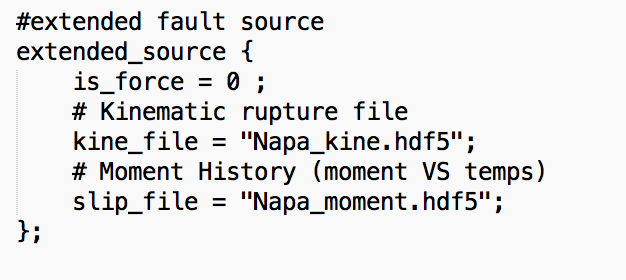
\includegraphics[scale=0.5]{figures/input-moment.png} 
\captionof{figure}{Extended source block in input.spec file for moment option.}
\label{sem} 
\vspace{1cm}
\end{center}



The first necessary information in 'extended source' block is the choice of force or moment-time history for the extended-source model. Here, we show the example of Napa bedrock case where we calculate moment-time history so that 'is\textunderscore force' parameter is set to 0. For force option, it should be set to 1. \\


Second, the name of file containing source properties such as coordinates should be given for 'kine\textunderscore file'. \\

Last, the name of file where moment-time history (or force-time history for force option) is stocked is specified as 'slip\textunderscore file'.


For Napa example, we provide the folder 'SEM\textunderscore extended\textunderscore source\textunderscore Napa\textunderscore rocher' folder. Even though we use a realistic model of fault plan, for simplicity, we prefer to define a single  type of soil in the propagation media. Once the simulation terminates, the procedure to analyze the outputs remain exactly the same as before. \\

















 
\bibliographystyle{apalike}
\bibliography {Biblio}

\end{document}
